\documentclass{article}

\usepackage{qtree}
\usepackage{graphicx}

\begin{document}
\title{Homework 12}
\date{}
\maketitle

% 1. Fall 09 Final, #2a
% 2. Textbook: 4.1.12

\paragraph{\Large 1. Fall 2009 Final Question 2a}\mbox{}\\
Run \textit{breadth-first search} on the graph below, starting adjacency sets are in sorted order, e.g., when exploring vertex \textit{F}, the algorithm considers the edge \textit{F-C} before \textit{F-D}, \textit{F-E}, or \textit{F-H}.\\

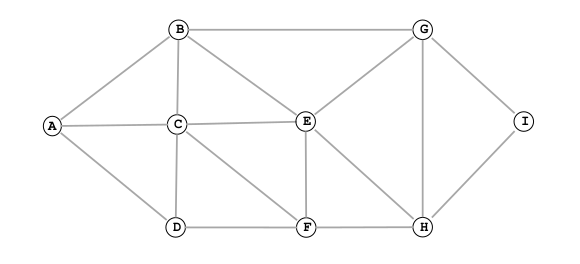
\includegraphics[width=\linewidth]{fin-f09-2a}\\

\noindent List the vertices in the order in which the vertices are enqueued on the FIFO queue.\\

A B C D E G F H I

\paragraph{\Large 2. Question 4.1.12}\mbox{}\\
What does the BFS tree tell us about the distance from v to w when neither is at the root?\\

The breadth-first search tree tells us the shortest path from v to w that passes through the root.

\end{document}